% Results deck: the Poisson 2D and Burgers 1D/2D results of the separable NM-ROM, as of
% 2026-09-04.  Companion to the study deck 2026-08-29-study-deck-linear-vs-nonlinear-residuals.tex
% (which explains the method); this one only shows the numbers.
% Every table is \input from tables/results-deck-*.tex, generated from the source reports'
% generated tables by reports/gen_2026-09-04-results-deck-tables.py.  Regenerate before building:
%   /home/tahmid/Dev/.venv/bin/python reports/gen_2026-09-04-results-deck-tables.py
%   latexmk -pdf -cd reports/2026-09-04-results-deck-burgers-poisson.tex
\documentclass[10pt,aspectratio=169]{beamer}
\usetheme{default}
\usecolortheme{default}
\setbeamertemplate{navigation symbols}{}
\setbeamertemplate{footline}[frame number]
\setbeamertemplate{itemize items}[circle]
\setbeamertemplate{blocks}[rounded][shadow=false]
\usepackage{amsmath,amssymb,bm}
\usepackage{booktabs}
\usepackage{tikz}
\usetikzlibrary{arrows.meta,positioning,fit,calc}
\usepackage{graphicx}
\usepackage{xcolor}

% --- palette (roles), same as the study deck ---
\definecolor{trained}{HTML}{C6531C}
\definecolor{trainedbg}{HTML}{FBE9E0}
\definecolor{frozen}{HTML}{2F5F8F}
\definecolor{frozenbg}{HTML}{E2ECF6}
\definecolor{solved}{HTML}{237A58}
\definecolor{solvedbg}{HTML}{DFF0E7}
\definecolor{plainbg}{HTML}{F7F7F2}
\definecolor{ink}{HTML}{152028}
\definecolor{accent}{HTML}{2F5F8F}

\setbeamercolor{structure}{fg=accent}
\setbeamercolor{title}{fg=ink}
\setbeamercolor{frametitle}{fg=ink}
\setbeamercolor{block title}{bg=frozenbg,fg=ink}
\setbeamercolor{block body}{bg=plainbg,fg=ink}
\setbeamercolor{block title alerted}{bg=trainedbg,fg=ink}
\setbeamercolor{block body alerted}{bg=plainbg,fg=ink}
\setbeamercolor{block title example}{bg=solvedbg,fg=ink}
\setbeamercolor{block body example}{bg=plainbg,fg=ink}
\setbeamerfont{frametitle}{series=\bfseries,size=\large}
\setbeamersize{text margin left=6mm,text margin right=6mm}
\setbeamertemplate{frametitle}{\vspace{2mm}\insertframetitle\par\vspace{1mm}}

\tikzset{
  box/.style={draw, rounded corners=2pt, align=center, font=\scriptsize, inner sep=4pt, minimum height=8mm},
  tr/.style={box, fill=trainedbg, draw=trained},
  fz/.style={box, fill=frozenbg, draw=frozen},
  sv/.style={box, fill=solvedbg, draw=solved},
  pl/.style={box, fill=plainbg, draw=gray!70},
  arr/.style={-{Stealth[length=2mm]}, thick, color=gray!60!black},
}
\AtBeginDocument{\setlength{\abovedisplayskip}{4pt}\setlength{\belowdisplayskip}{4pt}\setlength{\abovedisplayshortskip}{2pt}\setlength{\belowdisplayshortskip}{2pt}}

\newcommand{\T}{^{\top}}
\newcommand{\R}{\mathbb{R}}

\title{Separable NM-ROM: the Poisson and Burgers results}
\subtitle{Accuracy, cost per resolution, and where the ROM stands against the full-order solver}
\author{Tunable-NM-ROM project}
\date{4 September 2026 --- numbers final for these checkpoints (single seed, f64)}

\begin{document}

\begin{frame}
  \titlepage
  \begin{center}\scriptsize
    Every table is generated from the run JSONs (via the source reports named on each slide); nothing is typed by hand.\\
    Architecture slides are carried over from the 29 August study deck; the rest is the measured results.
  \end{center}
\end{frame}

% -------------------------------------------------------------------
\begin{frame}{What was measured, in one slide}
  \footnotesize
  \begin{columns}[T]
    \column{0.5\textwidth}
    \begin{block}{The model}
      A frozen decoder $u = G\,h(z)$ maps a small latent $z\in\R^{K}$ to the grid.
      The ROM solves the PDE for $z$ by driving a \emph{projected residual} $\Phi\T r(u)$ to zero, with $M$ test modes $\Phi$.
    \end{block}
    \begin{block}{The residual arms compared}
      \begin{itemize}
        \item \textbf{full / oracle}: residual summed on the whole grid --- the reference, cost $O(n)$.
        \item \textbf{sampled (NNLS, ``eq'', ``ex'')}: residual estimated at a few chosen points.
        \item \textbf{quadrature-free / tensor}: residual precomputed into a small table --- exact, no grid, no points.
      \end{itemize}
    \end{block}
    \column{0.5\textwidth}
    \begin{exampleblock}{The three questions each PDE answers}
      \begin{enumerate}
        \item \textbf{Accuracy} --- is the sample-free arm as accurate as the full grid?
        \item \textbf{Cost per resolution} --- does the ROM's time stay flat as the grid $N$ grows?
        \item \textbf{Against the FOM} --- at equal accuracy, is the ROM faster than a tuned classical solver?
      \end{enumerate}
    \end{exampleblock}
    \begin{alertblock}{How to read the numbers}
      Errors are relative $L_2$ against the full-order solution on held-out cases.
      Times are milliseconds per query (one Poisson solve, or one 50-step Burgers trajectory).
      ``Matched'' FOM = the cheapest classical tolerance setting that is at least as accurate as the ROM.
    \end{alertblock}
  \end{columns}
\end{frame}

% -------------------------------------------------------------------
\section{Architecture}


\begin{frame}{The separable decoder}
  \[
    u(x;z) \;=\; bc(x)\,\big\langle\, g(x),\; h(z)\,\big\rangle
    \;=\; bc(x)\sum_{j=1}^{R} g_j(x)\,h_j(z)
  \]
  \begin{columns}[T]
    \column{0.48\textwidth}
    \begin{itemize}
      \item $g(x)\in\R^{R}$ --- the \textbf{bank}: $R$ spatial \emph{shapes} (Fourier features $\to$ small MLP). Depends on $x$ only.
      \item $h(z)\in\R^{R}$ --- the \textbf{head}: MLP + linear skip from the latent to $R$ \emph{mixing amounts}. Depends on $z$ only.
      \item $bc(x)$ --- a fixed mask that makes the boundary condition hold exactly.
      \item $R=32$ (Burgers), $R=64$--$96$ (Poisson).
    \end{itemize}
    \column{0.52\textwidth}
    \begin{block}{Why ``separable'' matters}
      The two tracks never see each other's input. Evaluate the bank on any point set once and store it as a table
      \[
        G \in \R^{n\times R},\qquad G_{ij} = bc(x_i)\,g_j(x_i).
      \]
      Then the field on that point set is just
      \[
        u(z) \;=\; G\,h(z) \qquad(\text{table}\times\text{coefficient vector}).
      \]
      \textbf{The field is a mix of $R$ fixed shapes; only the $R$ mixing amounts depend on $z$.}
      Everything downstream exploits exactly this.
    \end{block}
  \end{columns}
\end{frame}

\begin{frame}{Architecture diagram --- who is trained, who is frozen, who is solved}
  \centering
  \resizebox{!}{0.72\textheight}{%
  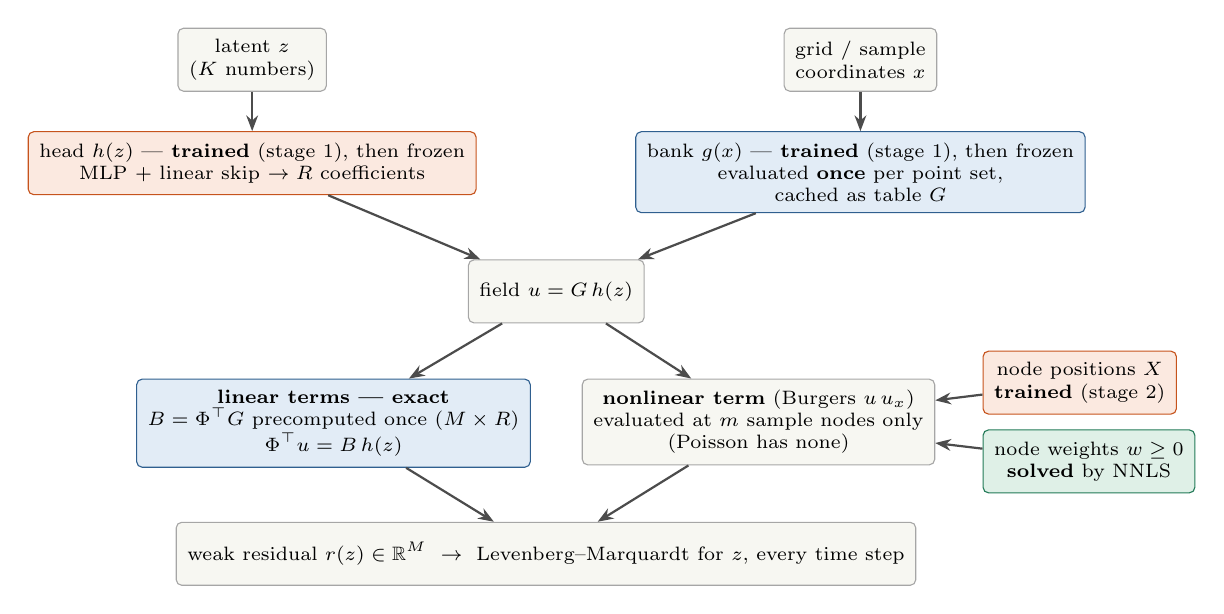
\begin{tikzpicture}[node distance=5mm and 9mm]
    \node[pl] (z) {latent $z$\\($K$ numbers)};
    \node[pl, right=58mm of z] (x) {grid / sample\\coordinates $x$};
    \node[tr, below=of z] (H) {head $h(z)$ --- \textbf{trained} (stage 1), then frozen\\MLP + linear skip $\to R$ coefficients};
    \node[fz, below=of x] (G) {bank $g(x)$ --- \textbf{trained} (stage 1), then frozen\\evaluated \textbf{once} per point set,\\cached as table $G$};
    \node[pl, below=7mm of $(H.south)!0.5!(G.south)$] (U) {field $u = G\,h(z)$};
    \node[fz, below left=7mm and -8mm of U] (LIN) {\textbf{linear terms --- exact}\\$B=\Phi\T G$ precomputed once ($M\times R$)\\$\Phi\T u = B\,h(z)$};
    \node[pl, below right=7mm and -8mm of U] (ADV) {\textbf{nonlinear term} (Burgers $u\,u_x$)\\evaluated at $m$ sample nodes only\\(Poisson has none)};
    \node[tr, right=6mm of ADV, yshift=5mm] (X) {node positions $X$\\\textbf{trained} (stage 2)};
    \node[sv, right=6mm of ADV, yshift=-5mm] (W) {node weights $w\ge0$\\\textbf{solved} by NNLS};
    \node[pl, below=7mm of $(LIN.south)!0.5!(ADV.south)$] (Rr) {weak residual $r(z)\in\R^{M}$ $\;\to\;$ Levenberg--Marquardt for $z$, every time step};
    \draw[arr] (z) -- (H); \draw[arr] (x) -- (G);
    \draw[arr] (H) -- (U); \draw[arr] (G) -- (U);
    \draw[arr] (U) -- (LIN); \draw[arr] (U) -- (ADV);
    \draw[arr] (X) -- (ADV); \draw[arr] (W) -- (ADV);
    \draw[arr] (LIN) -- (Rr); \draw[arr] (ADV) -- (Rr);
  \end{tikzpicture}}

  \vspace{2mm}
  {\scriptsize \textcolor{trained}{$\blacksquare$} trained by gradient \quad
   \textcolor{frozen}{$\blacksquare$} frozen / precomputed (exact path) \quad
   \textcolor{solved}{$\blacksquare$} solved by a convex fit, never gradient-trained}
\end{frame}

\begin{frame}{Stage 1 --- training the decoder (auto-decoder)}
  \[
    L_1 \;=\; \underbrace{\frac{\operatorname{mean}_s\,\|G\,h(z_s)-u_s\|^2}{\operatorname{mean}\,\|u\|^2}}_{\text{relative reconstruction}}
    \;+\; \lambda_{\mathrm{orth}}\,\underbrace{\Big\|\tfrac{G\T G}{n\,s^{2}}-I\Big\|_F^{2}}_{\text{keep the bank well-conditioned}}
  \]
  \footnotesize
  \begin{columns}[T]
    \column{0.55\textwidth}
    Jointly optimise the bank $g$, the head $h$, and \textbf{one latent code $z_s$ per training snapshot $u_s$}
    (there is no encoder --- the codes are free variables). $\lambda_{\mathrm{orth}}=10^{-4}$; Adam, full batch, warm-up then cosine decay ($10^{-3}\to10^{-5}$), 40\,000 steps.
    \column{0.45\textwidth}
    \begin{block}{In words}
      \begin{itemize}
        \item First term: ``every training snapshot must be reconstructible from \emph{some} 8-number code.''
        \item Second term: ``the $R$ shapes should be roughly orthogonal'' --- a conditioning nudge so the mixing amounts stay well-scaled; it does not change what the decoder can represent.
      \end{itemize}
    \end{block}
    \begin{alertblock}{After stage 1}
      Bank, head, and codes are \textbf{frozen}. Nothing downstream ever changes the decoder.
      The training codes are discarded; the solver finds its own $z$ at run time.
    \end{alertblock}
  \end{columns}
\end{frame}

\begin{frame}{How the decoder is used online --- it defines a manifold, it does not predict}
  \footnotesize
  \begin{columns}[T]
    \column{0.5\textwidth}
    \textbf{Weak form.} Pick $M$ test functions $\Phi\in\R^{n\times M}$ (sine modes = exact eigenvectors of the discrete Laplacian, $\Delta\Phi = \Phi\,\Lambda$). The residual handed to the solver is the PDE residual projected onto them:
    \[
      r(z) \;=\; \Phi\T\,\mathcal{R}\big(G\,h(z)\big)\;\in\R^{M},\qquad M = 32\text{ or }64 .
    \]
    \textbf{Solve.} Each time step: damped Levenberg--Marquardt over the $K$ latent unknowns, driving $r(z)\to0$; needs $r$ and $\partial r/\partial z$.
    \column{0.5\textwidth}
    \begin{block}{The cost question}
      $\Phi\T\mathcal{R}(u)$ is a \textbf{sum over all $n$ grid points}. Done naively, each of thousands of solver iterations would
      \begin{enumerate}
        \item decode $u=G\,h(z)$ on the grid ($n\times R$ flops),
        \item apply the PDE operator on the grid,
        \item sum against $M$ test modes.
      \end{enumerate}
      That is the full-order cost, every iteration.
    \end{block}
    \begin{block}{Two ways out}
      \textbf{Exact:} regroup the arithmetic so the grid disappears (works when the term is linear).\\
      \textbf{Approximate:} estimate the sum from $m\ll n$ sample points with weights --- \emph{quadrature} (needed when the term is nonlinear).
    \end{block}
  \end{columns}
\end{frame}

\begin{frame}{Poisson: the whole residual is a small table}
  \[
    \boxed{\;r(z) \;=\; W\odot\big[\,\Lambda\,B\,h(z) \;-\; f_M\,\big]\;}\qquad
    \frac{\partial r}{\partial z} \;=\; W\odot\Lambda\,B\;\frac{\partial h}{\partial z},\qquad B=\Phi\T G,\quad f_M=\Phi\T f
  \]
  \footnotesize
  \begin{columns}[T]
    \column{0.52\textwidth}
    Poisson: $-\Delta u = f$. Every term is linear in $u$.
    \begin{itemize}
      \item \textbf{Laplacian moved onto the test modes.} Because $\Delta\Phi=\Phi\Lambda$,
        $\;\Phi\T(\Delta u) = (\Delta\Phi)\T u = \Lambda\,\Phi\T u.$
        The operator becomes $M$ known numbers $\Lambda$ --- it never touches the field.
      \item \textbf{Source term} projected once: $f_M=\Phi\T f$.
      \item $\partial h/\partial z$: autodiff of a $16\!\to\!64$ MLP ($16\!\to\!96$ at $N=128$).
      \item $W$: fixed per-mode scaling that balances the rows.
    \end{itemize}
    \column{0.48\textwidth}
    \begin{block}{What runs online}
      \begin{itemize}
        \item the tiny head $h(z)$,
        \item a $64\times64$ matvec ($64\times96$ at $N=128$),
        \item the head's $64\times16$ Jacobian.
      \end{itemize}
      \textbf{No grid. No decode. No sample points. No fitted weights.}
      The field $G\,h(z)$ is formed once, at the very end, to write out the answer.
    \end{block}
    \begin{block}{What ``0 sample points'' means}
      The sampled (NNLS) path estimates the same $M$ numbers from 256 chosen points --- and gets them 5--8\,\% wrong at solutions. The quadrature-free path computes them exactly and does not need the points at all.
    \end{block}
  \end{columns}
\end{frame}

\begin{frame}{What we do for Burgers: exact linear terms + sampled advection}
  \small Backward-Euler step from $z^n$ to $z$; $N(u)=u\,u_x$ (sign-upwind); $m$ nodes $X$ with weights $w\ge0$; $\Phi_X,G_X$ = test modes and bank evaluated at the nodes:
  \[
    r(z) \;=\; W\odot\Big[\underbrace{B\big(h(z)-h(z^n)\big)}_{\text{time derivative, exact}}
    \;+\;\Delta t\Big(\underbrace{\Phi_X\T\big(w\odot N_X(G_X h(z))\big)}_{\text{advection, sampled at } m \text{ nodes}}
    \;+\;\underbrace{\nu\,\Lambda\,B\,h(z)}_{\text{diffusion, exact}}\Big)\Big]
  \]
  \begin{columns}[T]
    \column{0.5\textwidth}
    \begin{block}{The per-iteration cost}
      Decode at $m$ nodes only ($m\times R$), one upwind stencil on $m$ values, an $M\times m$ matvec, and the exact linear part. \textbf{Independent of the grid size $n$.} Measured: latent solve flat from $N=128$ to $4096$.
    \end{block}
    \column{0.5\textwidth}
    \begin{exampleblock}{Choosing the nodes: baseline = NNLS}
      Given positions $X$, weights are fit by non-negative least squares so the sampled term reproduces the exact full-grid term on training states. Convex, no gradients, always available as a fallback. Positions themselves are the free choice --- stage 2 learns them.
    \end{exampleblock}
  \end{columns}
\end{frame}

\begin{frame}{Architecture with the tensor --- what changes, what does not}
  \centering
  \resizebox{!}{0.62\textheight}{%
  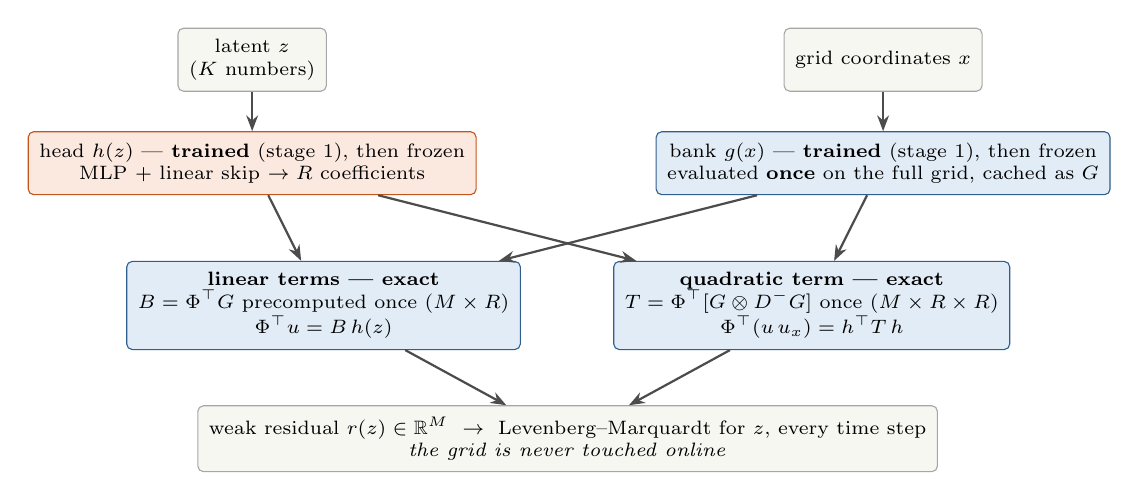
\begin{tikzpicture}[node distance=5mm and 9mm]
    \node[pl] (z) {latent $z$\\($K$ numbers)};
    \node[pl, right=58mm of z] (x) {grid coordinates $x$};
    \node[tr, below=of z] (H) {head $h(z)$ --- \textbf{trained} (stage 1), then frozen\\MLP + linear skip $\to R$ coefficients};
    \node[fz, below=of x] (G) {bank $g(x)$ --- \textbf{trained} (stage 1), then frozen\\evaluated \textbf{once} on the full grid, cached as $G$};
    \coordinate (mid) at ($(H.south)!0.5!(G.south)$);
    \node[fz] (LIN) at ($(mid)+(-31mm,-14mm)$) {\textbf{linear terms --- exact}\\$B=\Phi\T G$ precomputed once ($M\times R$)\\$\Phi\T u = B\,h(z)$};
    \node[fz] (TEN) at ($(mid)+(31mm,-14mm)$) {\textbf{quadratic term --- exact}\\$T=\Phi\T[G\otimes D^-G]$ once ($M\times R\times R$)\\$\Phi\T(u\,u_x) = h\T T\,h$};
    \node[pl, below=7mm of $(LIN.south)!0.5!(TEN.south)$] (Rr) {weak residual $r(z)\in\R^{M}$ $\;\to\;$ Levenberg--Marquardt for $z$, every time step\\\emph{the grid is never touched online}};
    \draw[arr] (z) -- (H); \draw[arr] (x) -- (G);
    \draw[arr] (H) -- (LIN); \draw[arr] (H) -- (TEN);
    \draw[arr] (G) -- (LIN); \draw[arr] (G) -- (TEN);
    \draw[arr] (LIN) -- (Rr); \draw[arr] (TEN) -- (Rr);
  \end{tikzpicture}}

  \vspace{2mm}
  \begin{columns}[T]
    \column{0.5\textwidth}\small
    \textbf{Training: nothing new.} Stage 1 is unchanged (same loss $L_1$, same 40\,000 steps, same checkpoints --- the results below reuse the \emph{committed} decoders, nothing retrained).
    \column{0.5\textwidth}\small
    \textbf{Stage 2 disappears.} No node positions to learn, no NNLS weights to fit, no budget $m$ to choose, no held-out monitoring. The orange ``nodes'' box and the green ``weights'' box of the earlier diagram are gone; the blue path is the whole residual, as for Poisson.
  \end{columns}
\end{frame}

\begin{frame}{After stage 1: what each case builds from the frozen decoder}
  \centering
  \resizebox{\textwidth}{!}{%
  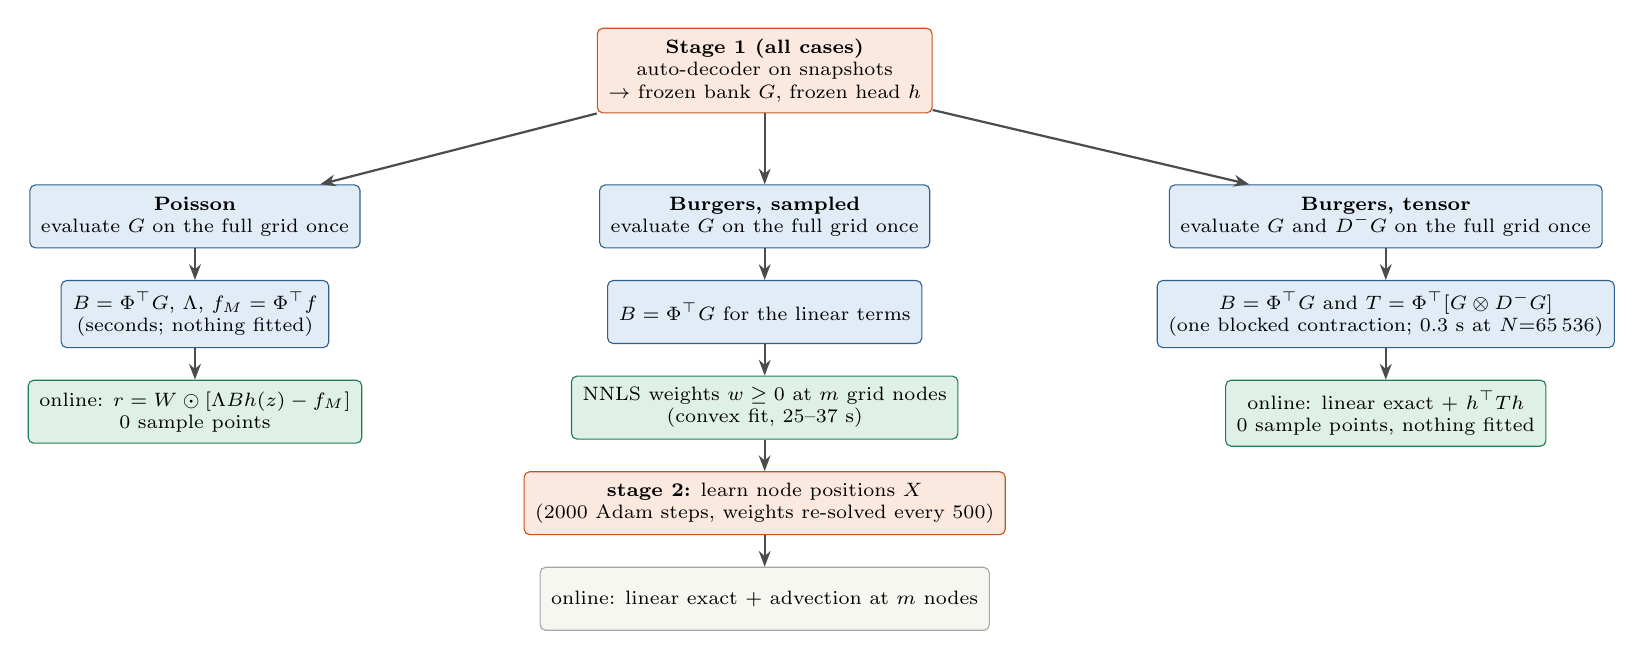
\begin{tikzpicture}[node distance=4mm and 6mm, every node/.style={font=\scriptsize}]
    \node[tr] (S1) {\textbf{Stage 1 (all cases)}\\auto-decoder on snapshots\\$\to$ frozen bank $G$, frozen head $h$};
    % Poisson column
    \node[fz, below left=9mm and 30mm of S1] (P1) {\textbf{Poisson}\\evaluate $G$ on the full grid once};
    \node[fz, below=of P1] (P2) {$B=\Phi\T G$, $\Lambda$, $f_M=\Phi\T f$\\(seconds; nothing fitted)};
    \node[sv, below=of P2] (P3) {online: $r=W\odot[\Lambda B h(z)-f_M]$\\0 sample points};
    % sampled column
    \node[fz, below=9mm of S1] (Q1) {\textbf{Burgers, sampled}\\evaluate $G$ on the full grid once};
    \node[fz, below=of Q1] (Q2) {$B=\Phi\T G$ for the linear terms};
    \node[sv, below=of Q2] (Q3) {NNLS weights $w\ge0$ at $m$ grid nodes\\(convex fit, 25--37 s)};
    \node[tr, below=of Q3] (Q4) {\textbf{stage 2:} learn node positions $X$\\(2000 Adam steps, weights re-solved every 500)};
    \node[pl, below=of Q4] (Q5) {online: linear exact $+$ advection at $m$ nodes};
    % tensor column
    \node[fz, below right=9mm and 30mm of S1] (T1) {\textbf{Burgers, tensor}\\evaluate $G$ and $D^-G$ on the full grid once};
    \node[fz, below=of T1] (T2) {$B=\Phi\T G$ and $T=\Phi\T[G\otimes D^-G]$\\(one blocked contraction; 0.3 s at $N{=}65\,536$)};
    \node[sv, below=of T2] (T3) {online: linear exact $+$ $h\T T h$\\0 sample points, nothing fitted};
    \draw[arr] (S1) -- (P1); \draw[arr] (S1) -- (Q1); \draw[arr] (S1) -- (T1);
    \draw[arr] (P1) -- (P2); \draw[arr] (P2) -- (P3);
    \draw[arr] (Q1) -- (Q2); \draw[arr] (Q2) -- (Q3); \draw[arr] (Q3) -- (Q4); \draw[arr] (Q4) -- (Q5);
    \draw[arr] (T1) -- (T2); \draw[arr] (T2) -- (T3);
  \end{tikzpicture}}

  \vspace{1mm}
  {\scriptsize \textcolor{trained}{$\blacksquare$} gradient training \quad
   \textcolor{frozen}{$\blacksquare$} one-time exact precomputation from the frozen bank \quad
   \textcolor{solved}{$\blacksquare$} convex fit / direct evaluation, no gradients}
  \vspace{1mm}

  \small The decoder training is the same in all three columns; the columns differ only in what is \emph{derived} from the frozen bank. Linear and quadratic terms are derived exactly; only a term that is neither needs the fitted (green) and learned (orange) steps of the middle column.
\end{frame}

% -------------------------------------------------------------------
\section{Poisson 2D}

\begin{frame}{Poisson 2D --- three residual paths through the same solver}
  \centering\scriptsize
  % GENERATED by reports/gen_2026-09-04-results-deck-tables.py -- do not edit by hand.

\begin{tabular}{@{}rlrrrrrr@{}}
  \toprule
  $N$ & residual path & sample pts & solve ms & solution err & resid.\ err vs full & grad.\ cos (min) & setup s\\
  \midrule
  128 & full grid & 15\,876 & 3.98 & 3.06e-2 & 0 (ref) & 1.000 & --- \\
  128 & sampled (NNLS) & 256 & 3.14 & 3.06e-2 & 7.88e-2 & -0.608 & 28.6 \\
  128 & \textbf{quadrature-free} & \textbf{0} & \textbf{2.93} & 3.06e-2 & \textbf{4.23e-14} & 1.000 & \textbf{0.9} \\
  \midrule
  256 & full grid & 64\,516 & 4.96 & 3.14e-2 & 0 (ref) & 1.000 & --- \\
  256 & sampled (NNLS) & 256 & 2.75 & 3.14e-2 & 6.21e-2 & -0.602 & 37.3 \\
  256 & \textbf{quadrature-free} & \textbf{0} & \textbf{2.68} & 3.14e-2 & \textbf{3.61e-14} & 1.000 & \textbf{0.7} \\
  \midrule
  512 & full grid & 260\,100 & 11.11 & 3.15e-2 & 0 (ref) & 1.000 & --- \\
  512 & sampled (NNLS) & 256 & 3.09 & 3.15e-2 & 5.50e-2 & -0.653 & 25.4 \\
  512 & \textbf{quadrature-free} & \textbf{0} & \textbf{2.87} & 3.15e-2 & \textbf{3.25e-14} & 1.000 & \textbf{0.8} \\
  \bottomrule
\end{tabular}

\vspace{1.5mm}
{\footnotesize Online solve ms per held-out source at $\tau=10^{-3}$, $K=16$; all three paths through the identical solver on one A100-80GB. Solution error = relative $L_2$ against the FOM; residual error = relative deviation of the projected residual from the full-grid value at the solver's solutions; grad.\ cos = worst cosine between the path's gradient and the full-grid gradient; setup = one-time build of the path (NNLS fit or the $M\times R$ product).}


  \vspace{2mm}
  \begin{columns}[T]
    \column{0.33\textwidth}\small
    \textbf{Same answer.} The solution error is identical down all three rows of each block: it is the decoder's floor, and the residual path does not touch it.
    \column{0.33\textwidth}\small
    \textbf{Exact, not sampled.} The quadrature-free residual agrees with the full grid to $\sim 10^{-14}$; the sampled rule is 5--8\,\% off and its gradient can point the wrong way.
    \column{0.33\textwidth}\small
    \textbf{Flat and free.} Full grid climbs 4 $\to$ 11 ms across $N$; quadrature-free stays under 3 ms, and its setup is under a second instead of a 25--37 s NNLS fit.
  \end{columns}
  \vspace{1mm}{\tiny Source: \texttt{2026-08-27-b1d-node-screening-and-poisson-qf.md}.}
\end{frame}

\begin{frame}{Poisson 2D --- the exactness gate}
  \centering\small
  % GENERATED by reports/gen_2026-09-04-results-deck-tables.py -- do not edit by hand.


\begin{tabular}{@{}rrrrr@{}}
  \toprule
  $N$ & resid.\ rel.\ max (random $z$) & grad.\ rel.\ max (random $z$) & resid.\ rel.\ max (at solutions) & gate failures\\
  \midrule
  128 & 1.33e-15 & 7.06e-16 & 9.99e-14 & 0 \\
  256 & 7.41e-16 & 1.12e-15 & 2.90e-13 & 0 \\
  512 & 7.34e-16 & 6.19e-16 & 1.37e-13 & 0 \\
  \bottomrule
\end{tabular}

\vspace{1.5mm}
{\footnotesize Gate Q: quadrature-free residual and gradient against the full grid, relative, in f64.}


  \vspace{4mm}
  \begin{columns}[T]
    \column{0.5\textwidth}\small
    Residual and gradient of the quadrature-free path were checked against the full grid at random latent states and at every solver solution. All at machine precision, zero failures.
    \column{0.5\textwidth}\small
    This is what ``no sample points'' means: the $M$ projected residual values are \emph{computed}, not estimated, so there is nothing to fit and nothing to get wrong.
  \end{columns}
  \vspace{1mm}{\tiny Source: \texttt{2026-08-27-b1d-node-screening-and-poisson-qf.md}.}
\end{frame}

\begin{frame}{Poisson 2D --- against the classical solver}
  \centering\small
  % GENERATED by reports/gen_2026-09-04-results-deck-tables.py -- do not edit by hand.


\begin{tabular}{@{}rrrrrrl@{}}
  \toprule
  $N$ & unknowns & ROM ms & ROM err & CG ms & CG err & who wins\\
  \midrule
  64 & 3\,844 & 2.06 & 3.75e-2 & 1.31 & 3.20e-2 & CG 1.6$\times$ \\
  128 & 15\,876 & 3.09 & 3.06e-2 & 3.75 & 1.70e-2 & \textbf{ROM 1.2$\times$} \\
  256 & 64\,516 & 2.54 & 2.89e-2 & 8.16 & 1.10e-2 & \textbf{ROM 3.2$\times$} \\
  512 & 260\,100 & 3.06 & 3.15e-2 & 26.36 & 7.10e-3 & \textbf{ROM 8.6$\times$} \\
  1024 & 1\,044\,484 & 3.50 & 3.48e-2 & 98.31 & 4.90e-3 & \textbf{ROM 28.1$\times$} \\
  \bottomrule
\end{tabular}

\vspace{1.5mm}
{\footnotesize $K=16$, held-out sources, $\tau=10^{-3}$, same job and GPU. CG = cheapest unpreconditioned conjugate-gradient tolerance rung at least as accurate as the ROM (cheapest rung if none qualifies).}


  \vspace{3mm}
  \begin{columns}[T]
    \column{0.5\textwidth}\small
    \textbf{The ROM is flat; CG is not.} ROM time stays at 2--3.5 ms from $N=64$ to $N=1024$ while conjugate gradient grows with the grid. The crossover is at $N=128$.
    \column{0.5\textwidth}\small
    \textbf{Two caveats, stated plainly.} The CG rung is \emph{unpreconditioned}, so these speedups are soft. And Poisson with constant coefficients has an exact spectral direct solve (0.64 ms at $N=1024$, error $7\times10^{-15}$) that beats both. The ROM's win is against \emph{iterative} solvers.
  \end{columns}
  \vspace{1mm}{\tiny Source: \texttt{2026-08-25-poisson-architecture-and-results.md}.}
\end{frame}

% -------------------------------------------------------------------
\section{Burgers 1D}

\begin{frame}{Burgers 1D --- the tensor arm lands on the full-grid oracle}
  \centering\scriptsize
  % GENERATED by reports/gen_2026-09-04-results-deck-tables.py -- do not edit by hand.


\begin{tabular}{@{}rrrrrr@{}}
  \toprule
  $N$ & full-grid (oracle) err & \textbf{tensor err} & $|$tensor$-$oracle$|$ max per traj & e2e oracle ms & \textbf{e2e tensor ms}\\
  \midrule
  128 & 5.01e-3 & \textbf{5.01e-3} & 1.2e-6 & 29.0 & \textbf{24.4} \\
  256 & 6.16e-3 & \textbf{6.16e-3} & 6.4e-7 & 35.0 & \textbf{29.2} \\
  512 & 4.88e-3 & \textbf{4.88e-3} & 2.4e-7 & 30.7 & \textbf{27.5} \\
  1024 & 5.54e-3 & \textbf{5.54e-3} & 2.3e-7 & 27.4 & \textbf{21.8} \\
  \bottomrule
\end{tabular}

\vspace{1.5mm}
{\footnotesize Rollout error = mean relative $L_2$ over 8 held-out trajectories $\times$ 51 states; e2e = end-to-end ms per 50-step trajectory (median of 8 traj $\times$ 5 reps), one A100, resolutions interleaved in one job.}


  \vspace{2mm}
  \begin{columns}[T]
    \column{0.33\textwidth}\small
    \textbf{Accuracy.} Tensor $=$ oracle per trajectory to $\le 1.2\times10^{-6}$, with zero sample points. Flat across $8\times$ in resolution.
    \column{0.33\textwidth}\small
    \textbf{Versus sampling.} NNLS-32 is 2--10\,\% worse than the oracle; learned-32 closes that gap. The tensor's gain here is exactness and simplicity, not a lower error.
    \column{0.33\textwidth}\small
    \textbf{Cost.} 22--29 ms end to end, within a few percent of the sampled rule and 10--20\,\% under the oracle. In 1D everything is launch-bound.
  \end{columns}
  \vspace{1mm}{\tiny Source: \texttt{2026-08-29-b1d-tensor-sample-free-burgers.md}.}
\end{frame}

\begin{frame}{Burgers 1D --- cost per resolution, and against the FOM}
  \begin{columns}[T]
    \column{0.48\textwidth}
    \centering\scriptsize
    % GENERATED by reports/gen_2026-09-04-results-deck-tables.py -- do not edit by hand.

\resizebox{\textwidth}{!}{%
\begin{tabular}{@{}lrrrr@{}}
  \toprule
  arm & $N$ range & solve ms & IC fit ms & e2e ms\\
  \midrule
  oracle & 128..4096 & -0.0374 & -0.0055 & -0.0322 \\
  tensor & 128..4096 & -0.0772 & -0.0011 & -0.0493 \\
  \bottomrule
\end{tabular}}

\vspace{1.5mm}
{\footnotesize Exponent $p$ in ms $\sim N^{p}$, least-squares fit of $\log$ ms against $\log N$ inside one job on one GPU.}

    \column{0.52\textwidth}
    \centering\scriptsize
    % GENERATED by reports/gen_2026-09-04-results-deck-tables.py -- do not edit by hand.

\resizebox{\textwidth}{!}{%
\begin{tabular}{@{}rrrrrr@{}}
  \toprule
  $N$ & ROM e2e ms & FOM ms & ROM/FOM & ROM ms/traj (batch of 8) & ROM err\\
  \midrule
  512 & 24.0 & 7.87 & 3.0$\times$ & 7.9 & 5.19e-3 \\
  4096 & 21.9 & 8.77 & 2.5$\times$ & 6.6 & 4.89e-3 \\
  \bottomrule
\end{tabular}}

\vspace{1.5mm}
{\footnotesize Optimised 1D rollout (learned 32 nodes) against the tridiagonal tolerance-Newton FOM at ntol $10^{-3}$. Not iso-accuracy: the FOM is more accurate at every $N$. The FOM was not batched.}

  \end{columns}

  \vspace{3mm}
  \begin{columns}[T]
    \column{0.5\textwidth}\small
    \textbf{Flat in $N$ --- and so is everything else.} Every arm's exponent is $\approx 0$ over $128\ldots4096$: below $\sim 10^{4}$ points the GPU time is kernel launches, not arithmetic. Flatness is real; a 1D crossover is not.
    \column{0.5\textwidth}\small
    \textbf{No 1D speedup.} The tridiagonal FOM solves a trajectory in $\sim 8$ ms and is more accurate; the single-query ROM is 2.5--3$\times$ slower. Only batched throughput (8 trajectories at once) brings the ROM to the FOM's per-trajectory time.
  \end{columns}
  \vspace{1mm}{\tiny Sources: \texttt{2026-08-29-b1d-tensor-sample-free-burgers.md}, \texttt{2026-08-28-b1d-rollout-optimization.md}.}
\end{frame}

\begin{frame}{Burgers 1D --- seeing it ($N=512$)}
  \centering
  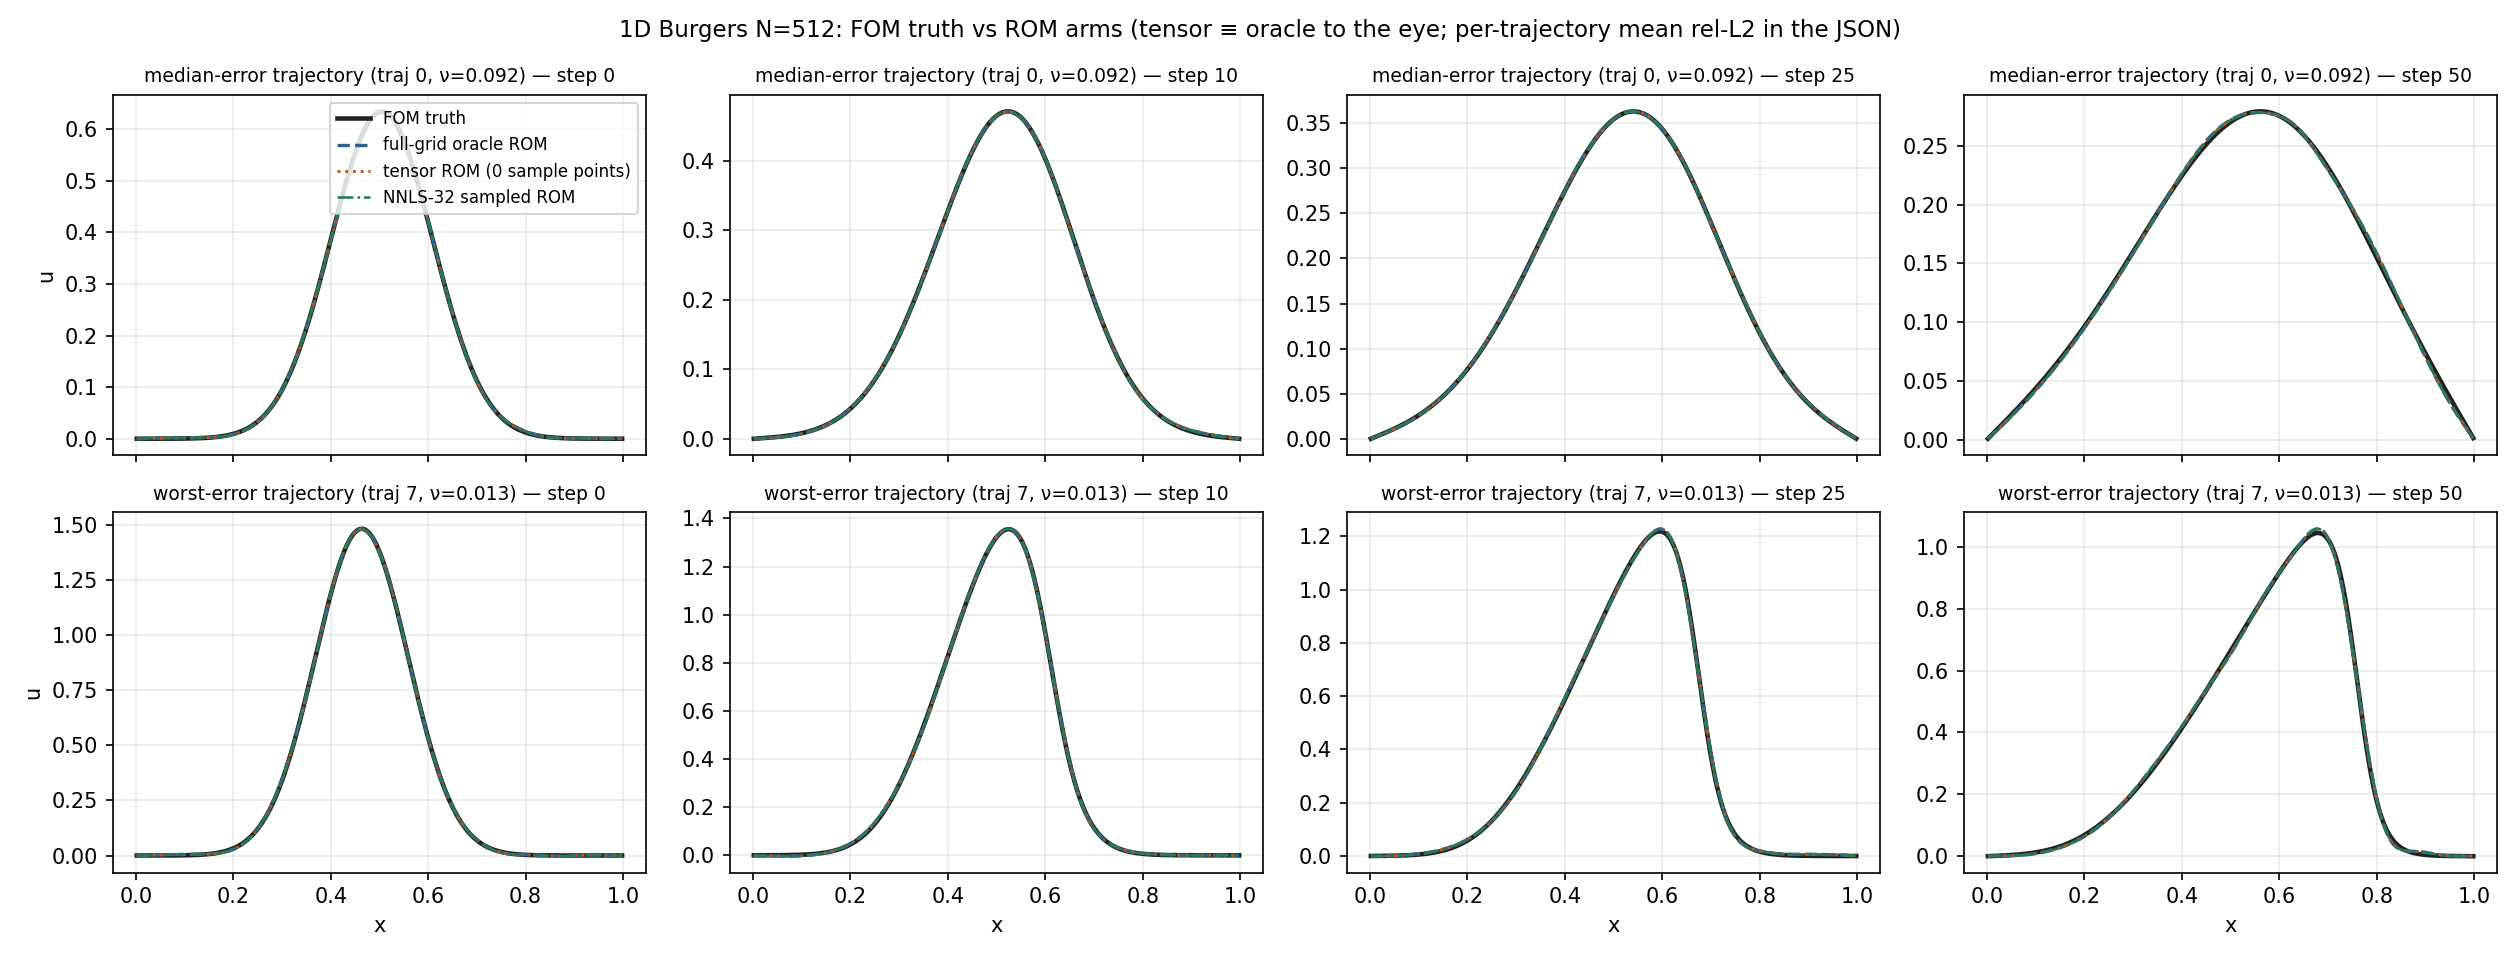
\includegraphics[width=0.9\textwidth,trim=0 0 0 40,clip]{figs/b1d-tensor-fields-n512.png}
  \vspace{0.5mm}\footnotesize
  FOM truth (black), full-grid oracle (blue dashed), tensor ROM (orange dotted) and NNLS-32 (green dash-dot) at steps 0/10/25/50; top the median-error trajectory, bottom the worst. All curves coincide at this scale.
\end{frame}

% -------------------------------------------------------------------
\section{Burgers 2D}

\begin{frame}{Burgers 2D --- accuracy per arm ($K=16$, $R=64$)}
  \centering\scriptsize
  % GENERATED by reports/gen_2026-09-04-results-deck-tables.py -- do not edit by hand.


\begin{tabular}{@{}rrrrrr@{}}
  \toprule
  $N$ & full-grid err & \textbf{tensor err} & $|$tensor$-$full$|$ max & tensor/full & same LM attempts\\
  \midrule
  64 & 2.31e-2 & \textbf{2.31e-2} & 7.9e-5 & 1.00033 & True \\
  256 & 2.45e-2 & \textbf{2.45e-2} & 7.3e-6 & 1.00003 & True \\
  512 & 2.46e-2 & \textbf{2.46e-2} & 1.9e-6 & 1.00001 & True \\
  1024 & 6.38e-2 & \textbf{6.38e-2} & 2.0e-5 & 1.00006 & True \\
  \bottomrule
\end{tabular}

\vspace{1.5mm}
{\footnotesize $K=16$, $R=64$, $M=64$. Rollout error = mean relative $L_2$ over 8 held-out trajectories $\times$ 51 states. \emph{full} = advection summed on the whole grid every iteration; \emph{tensor} = advection through the precomputed quadratic form.}


  \vspace{2mm}
  \begin{columns}[T]
    \column{0.33\textwidth}\small
    \textbf{Tensor $=$ full} at every $N$: same error to 5 digits, same stop reasons, same number of solver attempts.
    \column{0.33\textwidth}\small
    \textbf{Not better than sampling} at this budget (256 nodes for $M=64$ modes): sampling was never binding, so the tensor matches it with nothing fitted.
    \column{0.33\textwidth}\small
    \textbf{The $N=1024$ row} is a weaker inherited decoder; its $6.4\times10^{-2}$ is the checkpoint's floor, not the residual's.
  \end{columns}
  \vspace{1mm}{\tiny Source: \texttt{2026-08-30-b2d-tensor-ladder.md}.}
\end{frame}

\begin{frame}{Burgers 2D --- cost per resolution}
  \centering\scriptsize
  % GENERATED by reports/gen_2026-09-04-results-deck-tables.py -- do not edit by hand.


\begin{tabular}{@{}rlrrrrrr@{}}
  \toprule
  $N$ & \textbf{GPU} & full-grid solve & \textbf{tensor solve} & tensor/full & IC fit & decode & \textbf{tensor e2e}\\
  \midrule
  64 & A100-40 & 32.6 & \textbf{27.5} & 0.845 & 2.0 & 0.40 & \textbf{29.6} \\
  256 & A100-80 & 74.1 & \textbf{27.7} & 0.374 & 2.2 & 0.54 & \textbf{29.8} \\
  512 & H200 & 97.3 & \textbf{20.0} & 0.205 & 1.6 & 0.49 & \textbf{21.1} \\
  1024 & A100-80 & 670.0 & \textbf{27.1} & 0.040 & 4.8 & 1.15 & \textbf{32.6} \\
  \bottomrule
\end{tabular}

\vspace{1.5mm}
{\footnotesize Latent-solve ms per 50-step trajectory. \textbf{Each $N$ ran on a different GPU}: the ratios are measured inside one job and are sound; the raw ms across rows mix cards and are not an exponent.}


  \vspace{2mm}
  \begin{columns}[T]
    \column{0.5\textwidth}\small
    \textbf{The $O(n)$ arm moves; the tensor does not.} Full-grid solve climbs $33 \to 670$ ms over $16\times$ in resolution. The tensor stays at 20--28 ms, 2--8\,\% under the sampled rule, with a 2 s build instead of an 11--26 s NNLS fit.
    \column{0.5\textwidth}\small
    \textbf{Mixed hardware.} The four rungs ran on three different cards. Read the within-row ratios (tensor/full, tensor/ex); do not fit an exponent through the ms column.
  \end{columns}
  \vspace{1mm}{\tiny Source: \texttt{2026-08-30-b2d-tensor-ladder.md}.}
\end{frame}

\begin{frame}{Burgers 2D --- against the FOM at matched accuracy ($K=16$)}
  \centering\scriptsize
  % GENERATED by reports/gen_2026-09-04-results-deck-tables.py -- do not edit by hand.

\resizebox{\textwidth}{!}{%
\begin{tabular}{@{}rlrrrrrrrrr@{}}
  \toprule
  $N$ & GPU & tensor err & tensor e2e & matched FOM err & matched FOM ms & paired ROM ms & paired FOM ms & \textbf{speedup} & tightest FOM err & tightest FOM ms\\
  \midrule
  64 & A100-40 & 2.31e-2 & 29.6 & 3.75e-4 & 12.4 & 29.6 & 12.4 & 0.42$\times$ & 1.35e-4 & 16.3 \\
  256 & A100-80 & 2.45e-2 & 29.8 & 3.54e-4 & 17.3 & 29.5 & 17.2 & 0.58$\times$ & 1.33e-4 & 23.6 \\
  512 & H200 & 2.46e-2 & 21.1 & 3.51e-4 & 21.1 & 21.5 & 21.0 & 0.98$\times$ & 1.35e-4 & 27.4 \\
  1024 & A100-80 & 6.38e-2 & 32.6 & 2.97e-2 & 120.0 & 34.1 & 117.7 & \textbf{3.45$\times$} & 1.39e-4 & 230.7 \\
  \bottomrule
\end{tabular}}

\vspace{1.5mm}
{\footnotesize FOM = tolerance-Newton with the exact Helmholtz preconditioner, same GPU as the ROM. \emph{matched} = cheapest rung at least as accurate as the tensor arm; \emph{paired} = ROM and matched FOM timed alternately (AB/BA) in one job; \emph{tightest} = most accurate rung run.}


  \vspace{2mm}
  \begin{columns}[T]
    \column{0.5\textwidth}\small
    \textbf{A real crossover, at the finest grid only.} Below $N=1024$ the preconditioned Newton FOM reaches the ROM's accuracy in 12--21 ms and wins. At $N=1024$ its matched rung costs 118 ms and the tensor ROM is $3.45\times$ faster.
    \column{0.5\textwidth}\small
    \textbf{But the FOM is far more accurate when asked.} Its tightest rung reaches $\sim 1.4\times10^{-4}$ at every $N$, two orders below the ROM's floor. The ROM wins on time only at the accuracy its decoder allows.
  \end{columns}
  \vspace{1mm}{\tiny Source: \texttt{2026-08-30-b2d-tensor-ladder.md}.}
\end{frame}

\begin{frame}{Burgers 2D --- the larger sampled configuration ($K=32$, $R=512$)}
  \centering\small
  % GENERATED by reports/gen_2026-09-04-results-deck-tables.py -- do not edit by hand.


\begin{tabular}{@{}rlrrrrr@{}}
  \toprule
  $N$ & residual & GPU & rollout err & paired ROM ms & paired FOM ms & \textbf{ROM/FOM speed}\\
  \midrule
  256 & incumbent & A100-80 & 8.96e-3 & 43.9 & 16.4 & 0.37$\times$ \\
  256 & exact-linear & A100-40 & 8.02e-3 & 46.9 & 16.9 & 0.36$\times$ \\
  1024 & incumbent & H200 & 9.68e-3 & 33.2 & 63.2 & \textbf{1.90$\times$} \\
  1024 & exact-linear & H200 & 7.98e-3 & 33.6 & 62.9 & \textbf{1.87$\times$} \\
  \bottomrule
\end{tabular}

\vspace{1.5mm}
{\footnotesize $K=32$, $R=512$ (the larger, sampled configuration): matched-accuracy paired AB/BA against the swept Helmholtz-preconditioned Newton ladder. \emph{incumbent} = everything sampled by NNLS; \emph{exact-linear} = linear terms exact, advection sampled.}


  \vspace{3mm}
  \begin{columns}[T]
    \column{0.5\textwidth}\small
    \textbf{Lower error, same story.} With $K=32$ the rollout error drops to $\sim 8\times10^{-3}$. The ROM still loses at $N=256$ and wins about $1.9\times$ at $N=1024$.
    \column{0.5\textwidth}\small
    \textbf{Exact linear terms cost nothing.} Making the diffusion and time terms exact (``exact-linear'') lowers the error by 10\,\% and leaves the time unchanged. This configuration stays sampled: its $R=512$ bank does not compress into a tensor.
  \end{columns}
  \vspace{1mm}{\tiny Source: \texttt{2026-08-26-exact-linear-terms-and-gradient-eq.md}.}
\end{frame}

\begin{frame}{Burgers 2D --- seeing it ($N=256$)}
  \centering
  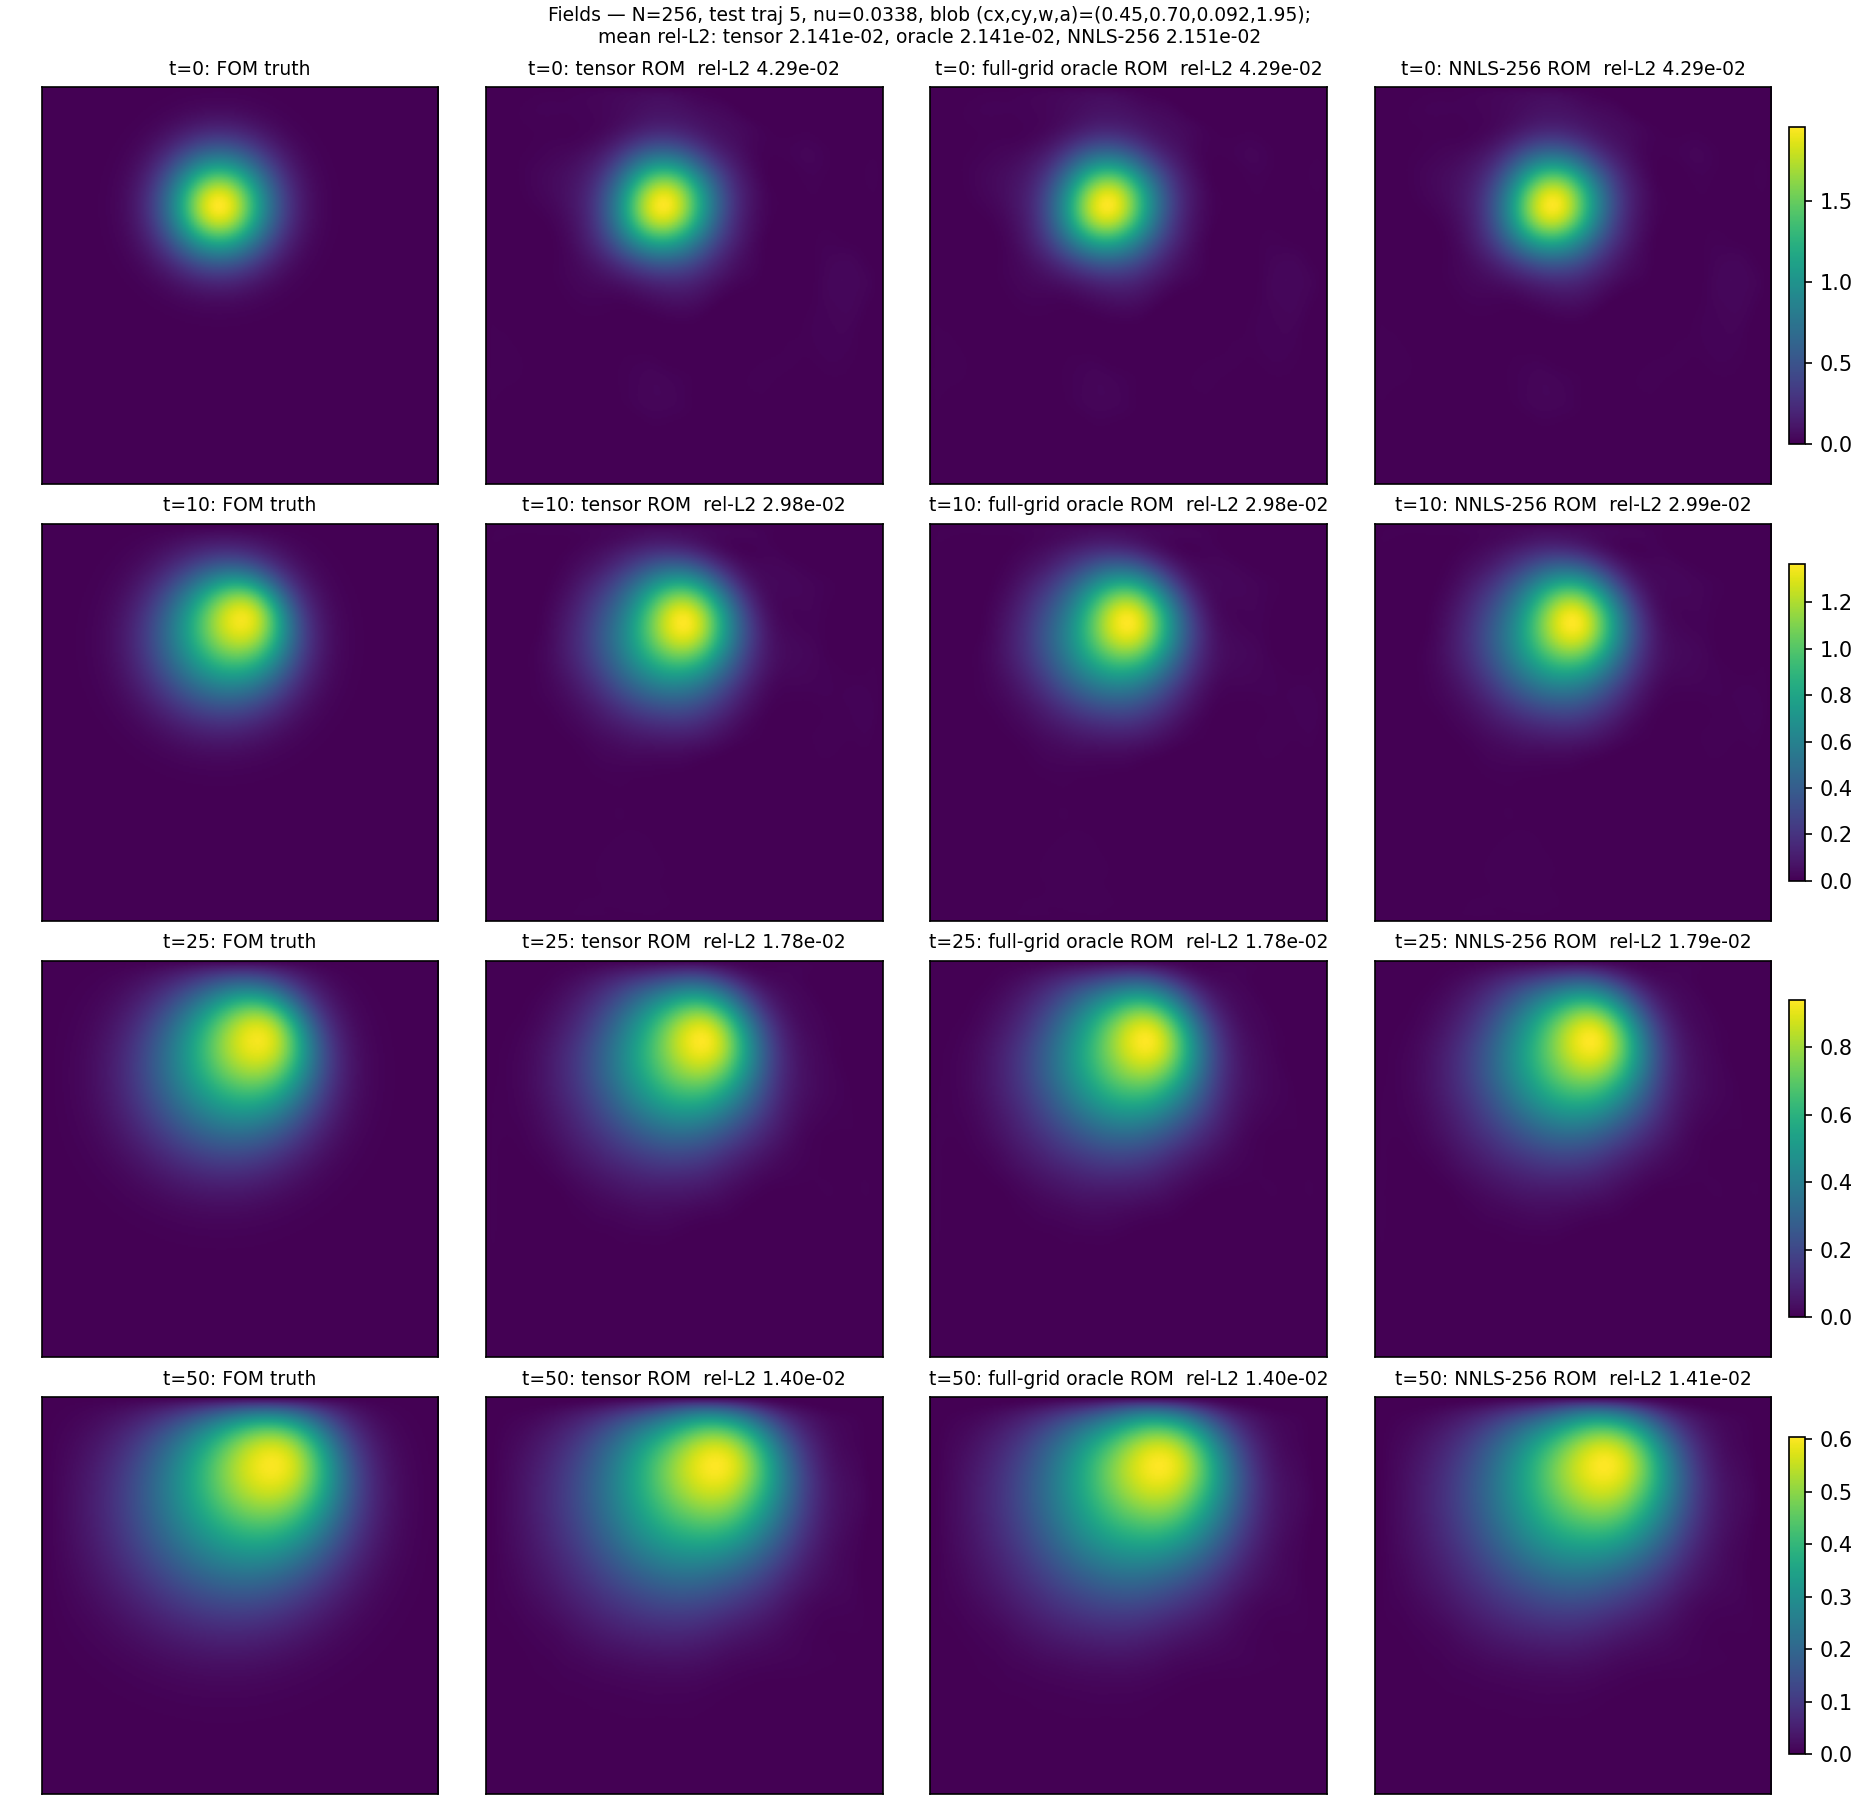
\includegraphics[height=0.74\textheight,trim=0 0 0 55,clip]{figs/b2d-tensor-fields_n256_traj5.png}\par
  \vspace{0.5mm}\footnotesize
  Truth and the three ROM arms (full, tensor, sampled) on one held-out trajectory; the arms are indistinguishable at this scale.
\end{frame}

% -------------------------------------------------------------------
\section{Summary}

\begin{frame}{The results in one table}
  \centering\small
  \begin{tabular}{@{}lp{0.27\textwidth}p{0.27\textwidth}p{0.27\textwidth}@{}}
    \toprule
    & \textbf{Accuracy of the sample-free arm} & \textbf{ROM cost vs $N$} & \textbf{Against the FOM at matched accuracy}\\
    \midrule
    \textbf{Poisson 2D} & $=$ full grid to $10^{-14}$; solution error unchanged & flat, $\sim 3$ ms & wins vs unpreconditioned CG from $N=128$; loses to the spectral direct solve\\
    \addlinespace
    \textbf{Burgers 1D} & $=$ full-grid oracle to $10^{-6}$ & flat, 22--29 ms (launch-bound) & loses 2.5--3$\times$ to the tridiagonal FOM at every $N$\\
    \addlinespace
    \textbf{Burgers 2D} & $=$ full-grid oracle to $10^{-5}$ & flat, 20--28 ms (full grid grows to 670 ms) & loses below $N=1024$; wins $3.45\times$ ($K=16$) / $1.9\times$ ($K=32$) at $N=1024$\\
    \bottomrule
  \end{tabular}

  \vspace{4mm}
  \begin{columns}[T]
    \column{0.5\textwidth}\small
    \textbf{What is established.} The precomputed residual (quadrature-free for linear terms, tensor for the quadratic one) reproduces the full-grid ROM exactly and makes the online cost independent of the grid.
    \column{0.5\textwidth}\small
    \textbf{What is not.} A speed win over a well-tuned classical solver exists only where the grid is large enough for the FOM to leave the launch floor: Burgers 2D at $1024^2$. Everything here is single-seed.
  \end{columns}
\end{frame}

\begin{frame}{Glossary}
  \footnotesize
  \begin{columns}[T]
    \column{0.5\textwidth}
    \begin{description}
      \item[FOM] full-order model: the classical solver on the whole grid.
      \item[ROM] reduced-order model: solves for the latent $z$ only.
      \item[$N$] grid points per side; unknowns $\approx N^2$ in 2D.
      \item[$K$, $R$, $M$] latent size, decoder bank width, number of test modes.
      \item[full / oracle] residual summed on the whole grid.
      \item[sampled / NNLS / eq] residual estimated at a few points chosen by non-negative least squares.
      \item[ex / exact-linear] linear terms exact, advection still sampled.
      \item[learned-32] sampled arm whose 32 node positions were trained.
    \end{description}
    \column{0.5\textwidth}
    \begin{description}
      \item[quadrature-free / tensor] residual precomputed into a small table; exact, no grid, no points.
      \item[e2e] end to end: initial-condition fit, latent solve, and final decode.
      \item[matched rung] cheapest FOM tolerance at least as accurate as the ROM.
      \item[paired / AB/BA] ROM and FOM timed alternately in one job on one GPU.
      \item[held-out] cases never seen in training.
      \item[CG] conjugate gradient, here unpreconditioned.
      \item[launch-bound] time dominated by GPU kernel launches, not arithmetic.
    \end{description}
  \end{columns}
\end{frame}

\end{document}
